\documentclass[paper=a4, fontsize=11pt]{article} % A4 paper and 11pt font size
%\usepackage[utf8x]{inputenc}
%\usepackage[czech]{babel} % English language/hyphenation
\usepackage{amsmath,amsfonts,amsthm} % Math packages
%\usepackage{lipsum} % Used for inserting dummy 'Lorem ipsum' text into the template
%\usepackage{sectsty} % Allows customizing section commands
%\allsectionsfont{\centering \normalfont\scshape} % Make all sections centered, the default font and small caps
\usepackage{fancyhdr} % Custom headers and footers
\pagestyle{fancyplain} % Makes all pages in the document conform to the custom headers and footers
\fancyhead{} % No page header - if you want one, create it in the same way as the footers below
\fancyfoot[L]{} % Empty left footer
\fancyfoot[C]{\thepage} % Empty center footer
\fancyfoot[R]{} % Page numbering for right footer
\renewcommand{\headrulewidth}{0pt} % Remove header underlines
\renewcommand{\footrulewidth}{0pt} % Remove footer underlines
\usepackage{graphicx}
\usepackage{indentfirst}
\usepackage[table]{xcolor}
\usepackage{booktabs}
\newcommand{\ra}[1]{\renewcommand{\arraystretch}{#1}}
\setlength\parindent{20pt} % Removes all indentation from paragraphs - comment this line for an assignment with lots of text
\usepackage{amssymb}
% Margins
\topmargin=-0.45in
\evensidemargin=0.0in
\oddsidemargin=-0.5in
\hoffset=1.0in
\textwidth=5.5in
\textheight=9.0in
\headsep=0.25in
%----------------------------------------------------------------------------------------
%	TITLE SECTION
%----------------------------------------------------------------------------------------

\newcommand{\horrule}[1]{\rule{\linewidth}{#1}} % Create horizontal rule command with 1 argument of height

\title{	
\normalfont \normalsize 
\textsc{Norwegian University of Science and Technology} \\ [25pt] % Your university, school and/or department name(s)
\horrule{0.5pt} \\[0.4cm] % Thin top horizontal rule
\huge Using Minimax with Alpha-Beta pruning to play Quarto\\ % The assignment title
\horrule{2pt} \\[0.5cm] % Thick bottom horizontal rule
}

\author{Jan Bednarik\\Tomas Dohnalek} % Your name

\date{\normalsize\today} % Today's date or a custom date

\begin{document}

\maketitle % Print the title

\section{Introduction}
\section{State evaluation function}
\section{Results}
\subsection{Random versus Novice}

\begin{table*}[h]\centering
\ra{1.3}
    \caption{Random against Novice player results. 100 Games.}.
\vspace{2mm}
\begin{tabular}{cccc}\toprule
Player type & Victories & Looses & Draws \\ \midrule
Random      & 3         & 97     & 0 \\
Novice      & 97        & 3      & 0 \\
\bottomrule
\end{tabular}
\label{tab:precedence}
\end{table*}


\begin{figure}[htp] \centering{
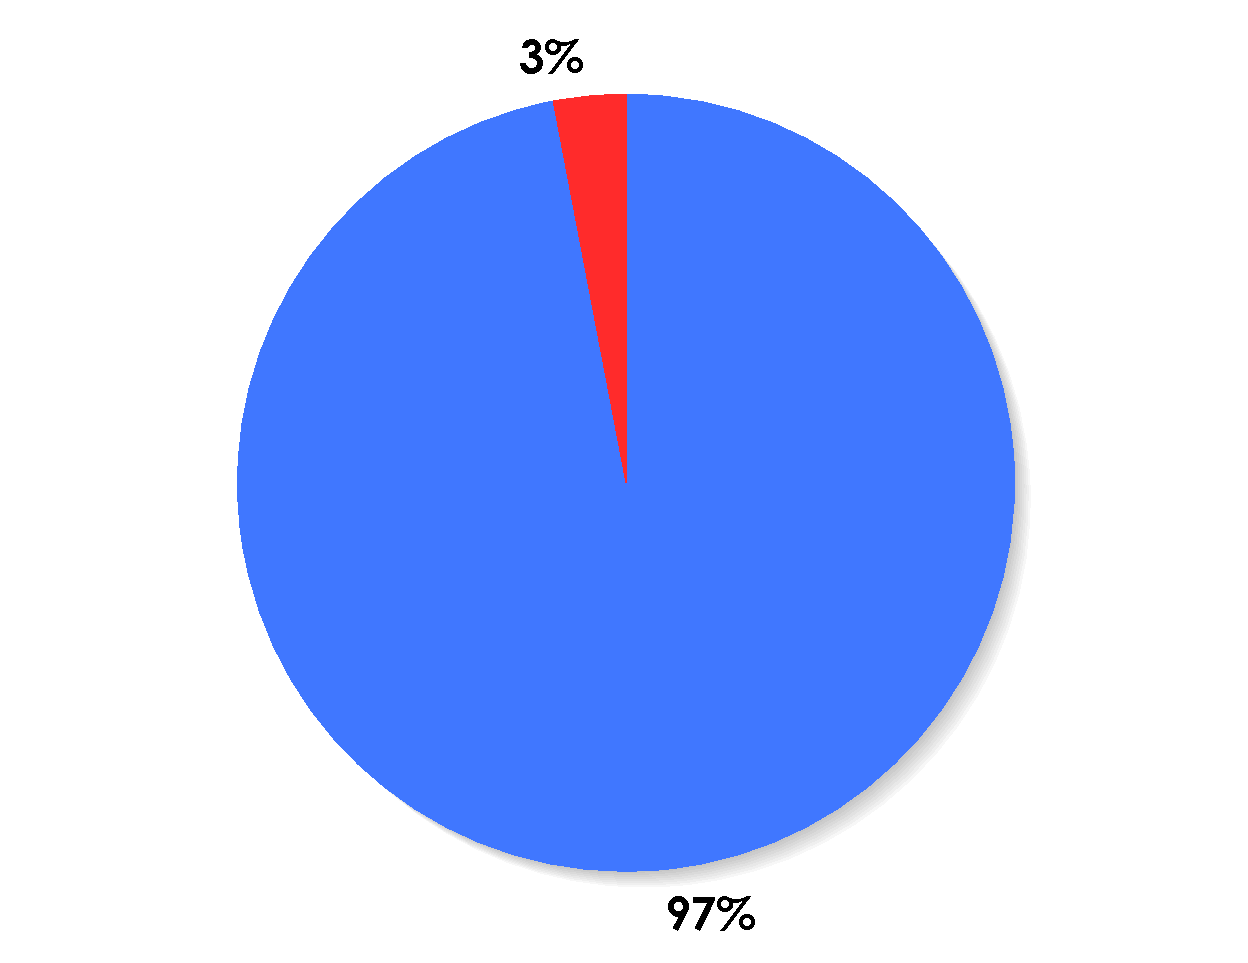
\includegraphics[scale=0.82]{img/random-novice.pdf}}
\caption{Random against Novice from Novice's point of view: \textcolor{blue!100!yellow!100!red!80}{$\bullet$} Victories, \textcolor{red!100}{$\bullet$} Looses.}
\end{figure}  

\subsection{Novice versus Minimax-3}
\subsection{Minimax-3 versus Minimax-4}
\subsection{Minimax in tournament}
\section{Participation in tournament}
\section{Summary}
%-----------------------------------------------
\begin{flushleft}
%\bibliography{literatura} % viz. literatura.bib..
%\bibliographystyle{czplain}
\end{flushleft}
\end{document}
